%==============================================================================%
\section{Research Themes} \label{section:literature:themes}
%==============================================================================%

In this section we look at the major themes and questions tackled by this knowledge base.
We start by classifying the research into the major and minor themes explored in them as shown in Figure \ref{figure:literature:themes}.
The tree-map shows the volume of research in corresponding themes measured in terms of number of publications.
We can observe that the research is conducted in five major areas - population studies focussing on the creating and utilising data on distribution and nature of human activity, mobility and interaction focussing on the changes in these distributions, understanding the nature and function of space from these distribution and change, methods and techniques which can be used to conduct the research and finally issues and solutions related to the privacy of the users while conducting these research.
We can also observe that most of the research apart from developing methods were conducted in the domain of human mobility and social interaction closely followed by the population distribution.
In the following sections we discuss these in detail along with their sub themes with the following framework,

\begin{enumerate}
  \setlength{\itemindent}{2em}
  \itemsep-0.25em
  \item What are the major lines of questioning?
  \item What has been done previously?
  \item Where are the opportunities for further research?
\end{enumerate}

\begin{figure}
  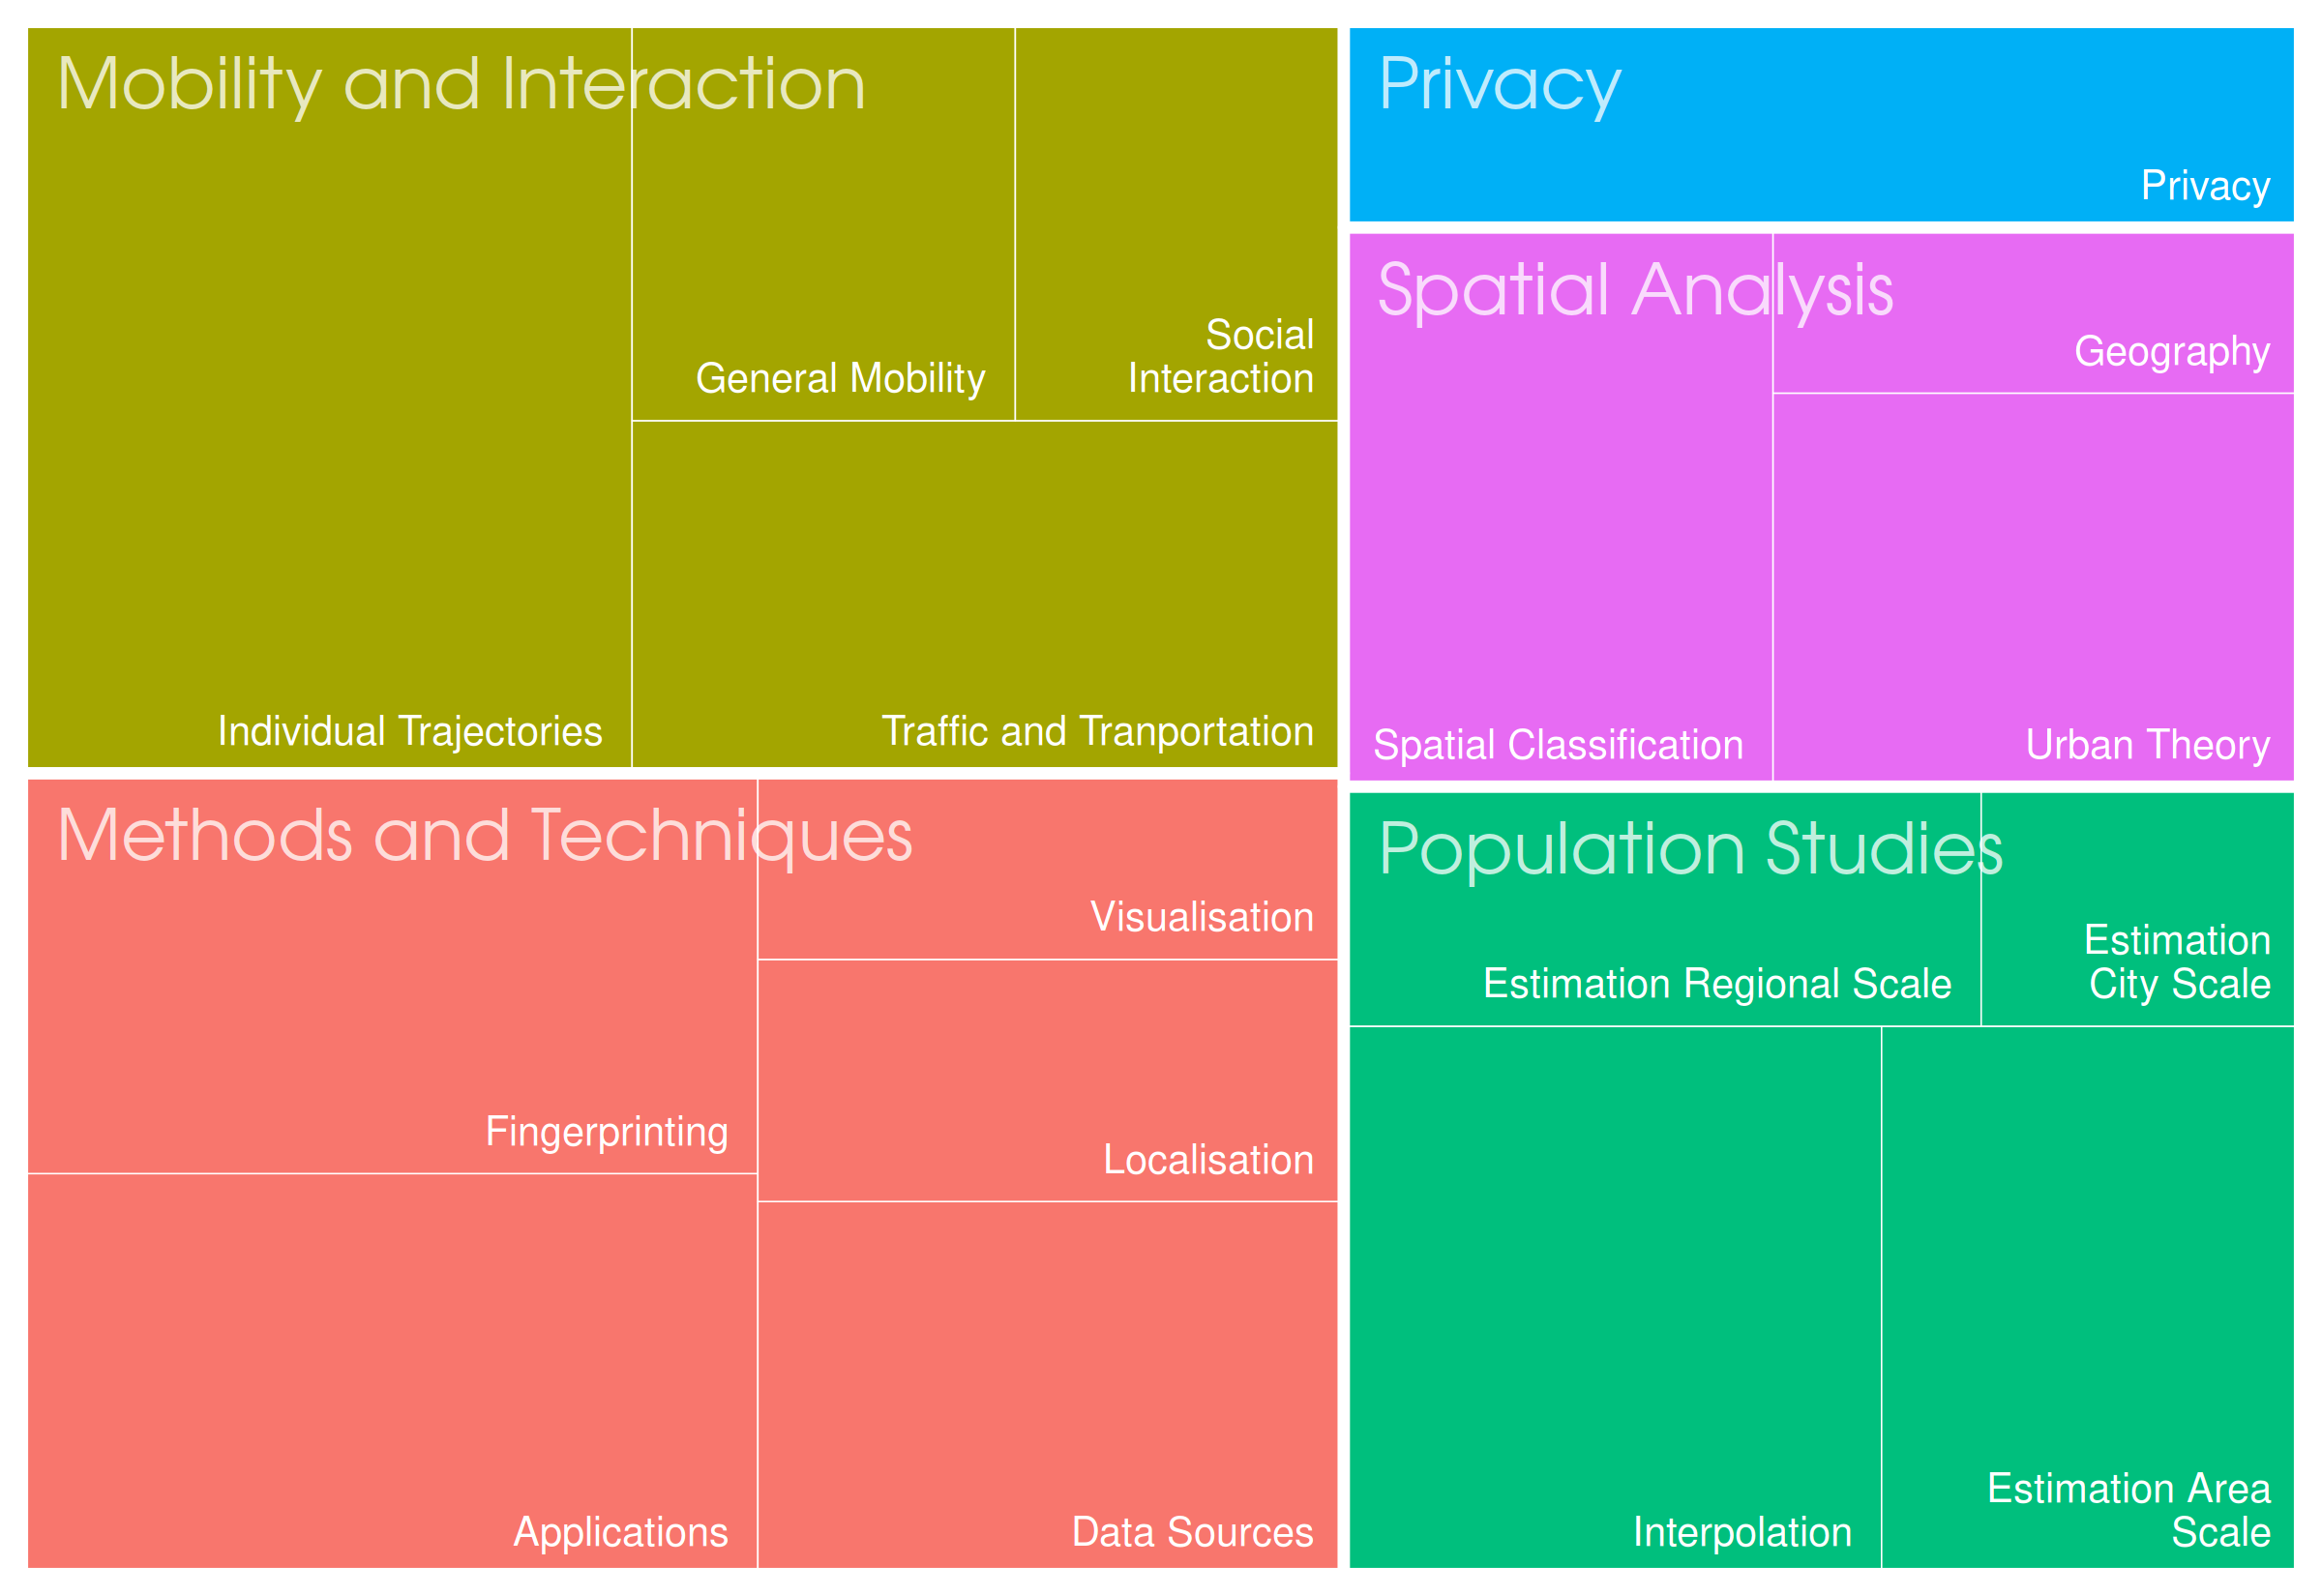
\includegraphics{images/literature-themes-treemap.png}
  \caption{Tree-map showing the volume of research conducted under each major themes and their sub-themes.}
  \label{figure:literature:themes}
\end{figure}
\marginnote[-2cm]{\textit{Measured by the number of publications.}}

%------------------------------------------------------------------------------%
\subsection{Population Studies}
%------------------------------------------------------------------------------%

Though \citet{foley1954} and \citet{schmitt1956} started this line of research in 1950's with the discussion on estimating daytime population using broader datasets it was not until the 80s significant volume of research kicked off in this area of study.
From 80s until mid 2000's numerous studies were conducted on measuring and studying the population at a granular level both spatially and temporally.
The focus of the research around this time was primarily on interpolation from the larger datasets created using censuses, regional or national level sample surveys and other centrally collected sources of data.
There have been numerous fairly successful attempts with methodologies where a broad dataset such  as regional level population summaries and modelling or interpolating more granular data from them by augmenting with other sources of data such as street networks \citep{reibel2005}, remote sensing \citep{sutton1997, yuan1997, chen2002} etc.
\citet{dobson2000, dobson2003a, bhaduri2002, bhaduri2007} and \citep{mennis2003, mennis2006} are examples of such research methodology.
These studies were almost done on a city scale or above with mostly modelling or interpolation methods since the data sources were few and were centrally collected.

Around 2005, there was a sharp shift in research where the interpolation methods were replaced by highly available granular data collected over cellular network.
Studies were conducted on estimating population densities, presence of tourists, general activity pattens using data from cellular networks.
Most of these research were conducted at a far larger geographic scale looking at things at an area level \citep{pulselli2008, girardin2009, phithakkitnukoon2010, yuan2016}.
There were efforts in using device level sensors such as global positioning system(GPS), Wi-Fi and Bluetooth to detect population distribution and socio-geographic routines \citep{calabrese2010, rose2010, farrahi2010}.
There have been studies on looking at people distribution as granular as queue lengths as discussed by \citep{wang2013} to city level dynamic population mapping where the limitations of traditional datasets generated through censuses and surveys \cite{deville2014}.

Around the 2015, along with the data collected directly from the mobile devices,the data that are generated by the users activity on these devices are became more important.
Social media data such as twitter \citep{lansley2016a} and other consumer data such as loyalty cards \citep{lloyd2018}, smart cards \citep{ordonez2012} etc. have also become a significant sources of data for such research.
Recently, with increased concerns and legislation on privacy, there have been studies which go back to the effort of interpolating granular data from broader datasets but using more data and processor intensive technologies such as agent based modelling, deep learning, small area estimation \citep{crols2019, shibata2019, rao2015} etc..
Though there have been a lot of work done in most of the directions in this research area, the clear gap arises due to the absence of a continuous, granular and sufficiently longitudinal data-sets to complement the methodologies that have been developed. 

%------------------------------------------------------------------------------%
\subsection{Human Mobility and Interaction}
%------------------------------------------------------------------------------%

Study of movement of people is one of the major areas of research which have significantly benefited from the decentralised collection of data at a granular level \cite{castells2000}.
In addition to being useful in their own right, these data were in turn used to augment traditional models of travel behaviour, traffic and transport to provide a better understanding of human movement over time and space \citep{janssens2013}.
The major themes of research within this area are, Movement of people in space and time with emphasis on understanding the built environment, social interaction between these people with a sociology perspective and traffic and transportation studies with a infrastructure perspective.
There is significant volume of research which dealt with recording and analysing the trajectories of the users to understand their movement patterns enabled by the unprecedented availability of detailed data from mobile devices and this is discussed in detail along with the discussion of the technologies used in Section \ref{section:literature:technology}.


%------------------------------------------------------------------------------%
\subsection{Methodology and Techniques}
%------------------------------------------------------------------------------%

Research in this are focused around 5 major topics,

\begin{enumerate}[rightmargin=2em, leftmargin=2em]
  \itemsep-0.25em
  \item Localisation - Research into using the mobile devices and data generated from them as a cheaper alternative to Global Positioning Systems and remote sensing.
  \item Data Sources - Identifying and formalising new data-sources as the technology develops
  \item Application - Applying these identified data sources to answer questions and solve problems in different disciplines.
  \item Visualisation - simplifying, visualising and interpreting these high volume of unstructured, noisy datasets.
  \item Device fingerprinting - overcoming the difficulties posed by the anonymisation process and extract useful information.
\end{enumerate}

Localisation of mobile devices without the use of expensive additional infrastructure such as GPS is one of the earliest ideas pursued in this aspect \citep{bulusu2000, he2003, moore2004, lamarca2005}.
This research, when reversed, could also lead to the tracking of these devices in space without the aforementioned infrastructure thus providing a inexpensive, easy way to collect mobility data.
The sensors which are already present in the phones such as Bluetooth \citep{bandara2004}, Wi-Fi \citep{zarim2006}, cellular radio \citep{dil2011, ahas2005} etc. have been considered to be used for localisation of the devices.
This has been particularly important in the field of indoor localisation where GPS doesn't usually work \cite[-2cm]{kawaguchi2009}.
When seen from the other perspective the same technologies and methods can enable us to collect presence and movement data on people indoors \citep{roy2018a, roy2018b, jia2019, nikitin2019, kulshrestha2019, deng2018}.

The identification of data sources started with looking at the 'real time' city examining the digital landscape created by the citizens their electronic devices \citep{townsend2000}.
This was furthered by the notion of `instrumenting' the city and developing methods and techniques under the umbrella of smart cities and internet of things \citep{oneill2006, sruthi2019}.
Since there have been research looking at the wireless data collected from positioning technologies \citep{bensky2007} and cellular network \citep{kiukkonen2010, steenbruggen2015} and even crowdsourcing as method of collection \citep{shin2013} leading towards a framework for computational urban planning \citep{kontokosta2015}.
With the effort to formalise them as valid sources of data, there have also been research looking at the biases in them such as mobile phone ownership \citep{wesolowski2013, kobus2013}.

Identifying and fingerprinting unique devices and users from noisy, unstructured data is another area of active research under methodologies and techniques \cite{jiang2006, liao2006}.
The majority of the work has been done as an extension of localisation where the GPS-less positioning leading to finger printing people and their movement out of the data \citep{pang2007a, pappalardo2015}.
Additionally there are work looking at the tracks collected from Wi-Fi or mobile data and extract unique users out of them \citep{girardin2008, eagle2009, jiang2012}.
It is also demonstrated that it is possible to wireless technologies can be used to detect even device free entities \citep{elgohary2013}.
These localisation and clustering techniques can also be used for socio-geographical analysis and to understand the patterns of activity of people \citep{licoppe2008}.
There has been a good deal of security research on the robustness of the anonymisation techniques while revealing methodologies to overcome limitations imposed by them \citep{mathieucunche2016, chothia2010, krumm2007}.
\citet{cheng2016} was one of the first to look into devising a method to do this in a non-intrusive way which are further extended by \citet{di2016, adamsky2018} and \citet{dai2019}.
This is currently an active field of research and there is immense opportunity for further research.

Visualising the temporal dynamics of data collected on human activities through decentralised processes poses significant challenges when approached with traditional cartographic concepts \cite{maceachren2001, hallisey2005}.
Digital media especially animation has been explored as an option to solve for the temporal dimension \citep{morrison2000, lobben2003} but is bound by the cognitive limits of the viewer \citep{harrower2007}.
There have been approaches proposed around animations of generated surfaces \citep{kobayashi2011} and network-based visualizations \citep{ferrara2014} leaving gaps in research for new methods in dynamic geographic visualisation \citep{fabrikant2005} and visualising path and flow of phenomena \citep{thomas2005}, particularly of the mobility data collected from cellphones \citep{sbodio2014}.
This provides us with a promising opportunity for research in methods for visualising high frequency, hyper-local pedestrian data within the limits of cognition of the viewer.

%------------------------------------------------------------------------------%
\subsection{Spatial Analysis - Theory and Modelling}
%------------------------------------------------------------------------------%

Traditional and modern geography was dominated by the study of centrally collected data acquired through extensive field surveys and remote sensing.
In the last two decades, a significant paradigm change has been introduced by the availability of unprecedented amount of data generated by unconventional sources such as mobile phones, social media posts etc.
This move to the postmodern geography has been accompanied by a change in our understanding of the built environment and human geography from a static point of view to a more dynamic definition \cite{soja1989}.
This definition is based on the bottom-up mechanisms which make human activity such as information exchange and economy to manifest in the physical built environments as argued by \citep{batty1990, batty1997, batty2012} and \citep{batty2013, batty2013a}.

This transition into the digital age \citep{graham1999, tranos2012, tranos2013} has changed the politics of space and time \citep{massey1992} and been more pronounced in the study of urban built environment where technology has redefined the concepts of place and space \citep{graham2001, graham2002, sassen2001}.
With the ability to collect and analyse of data on large complex systems in real-time \citep{graham1997}, we are exploring the possibilities of understanding their structure and organisation using concepts of complexity theory \citep{bettencourt2013, portugali2012} with more emphasis on their temporal patterns such as the argument towards finding the pulse of the city \citep{batty2010}.
With the population getting more and more connected \citep{castells2010}, the nature of space/place is being dynamically defined by the population themselves \citep{giuliano1991} and vice versa \citep{zandvliet2006}.
This flood of hard data \cite{nature2008} was accompanied not only by optimism in its potential \citep{thomas2001} but also by the questions raised on the challenges in handling the diverse, large scale, non standardised data it produces and the usefulness or representativeness of the resulting analysis \citep{miller2010, arribas-bel2014a}.
However, availability of such data has impressive uses in urban studies \citep{bettencourt2014} especially with advancement of new technologies \citep{steenbruggen2013} and possibility of distributed, crowdsourced data collection \citep{lokanathan2015}.

%------------------------------------------------------------------------------%
\subsection{Privacy}
%------------------------------------------------------------------------------%

The ubiquity of personal devices and digitisation of day to day activities through these mobile devices \citep{mcmeel2018} has provided many opportunities for researchers and industry for collecting, analysing and deriving inputs from them.
However at the same this also increased the risk of infringement on privacy of the users whose data is being collected \cite[-2cm]{saponas2007, krumm2009}.
There is immense value in uniquely identifying and profiling information on people for specialised purposes such as security \citep{cutter2006} and law enforcement \citep{dobson2003} but also has extreme risks associated when not handled with care \citep{vanwey2005}.
Strictly protecting personal information while ensuring the information is usable for research by maintaining the uniqueness in the data is the major concern which was addressed by devising frameworks for secure practices in confidentially collecting and using the location data \citep{duckham2006, tang2006, lane2014}.  Some efforts sought to accomplish this task through cryptographic hashing algorithms (Pang, 2007) while others aimed to thwart identification and tracking at the device level by techniques such as MAC randomisation \citep{gruteser2005, greenstein2008}.
Finally though getting consent of users for the collection and use of such information from their mobile devices is challenging, there is a significantly improved acceptance when the process offers value in return such as discounts and monetary benefits \citep{kobsa2014}.

There is opportunity in this area for research in applying the cryptographic solutions along with the privacy preserving frameworks to arrive at methods which can extract useful information out of large personal data while obscuring or anonymising them.

%==============================================================================%
\section{Research Trends}
%==============================================================================%

\begin{figure*}
  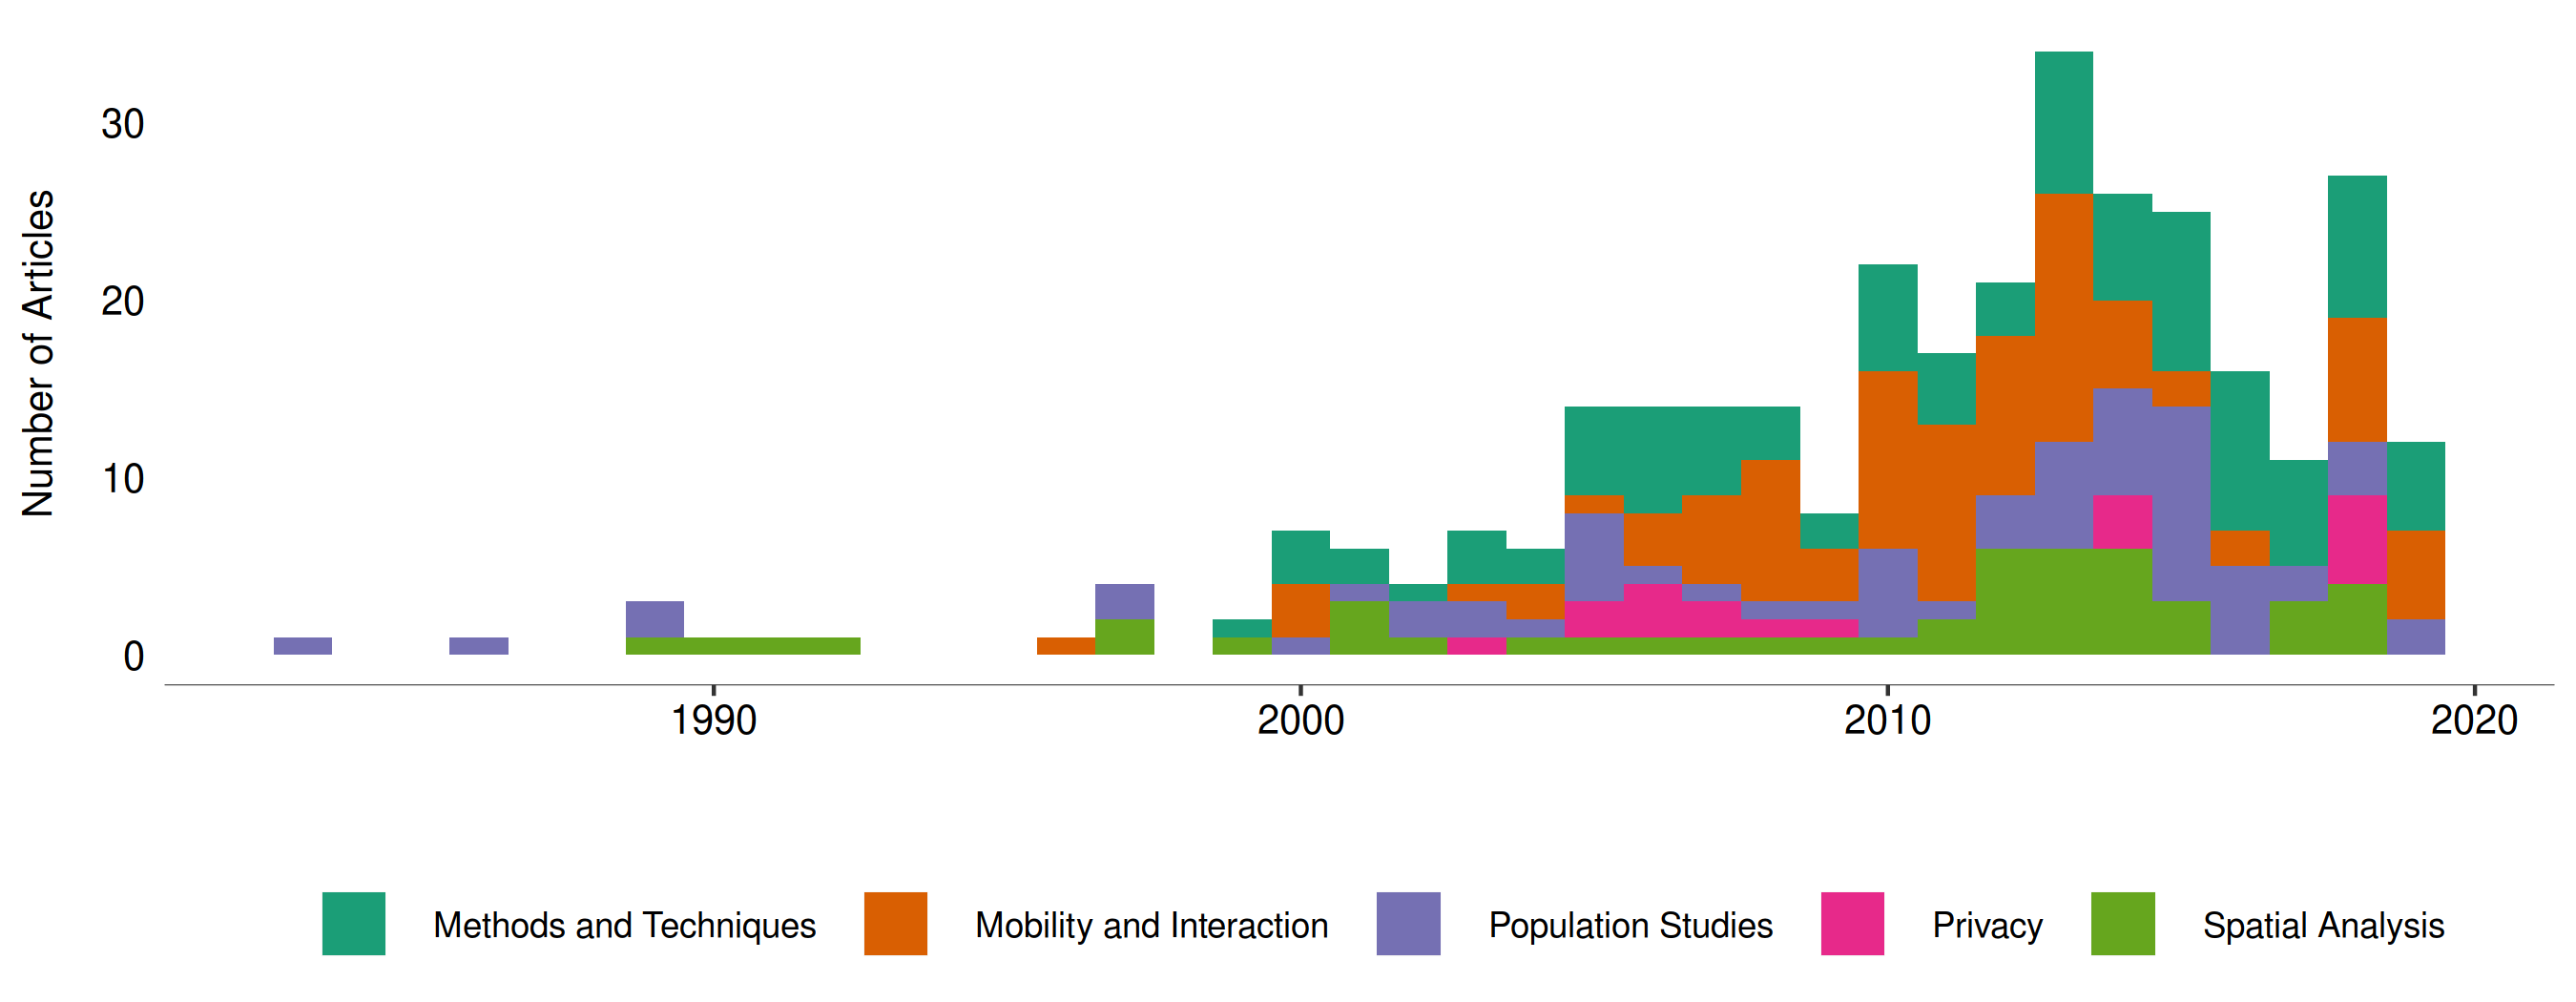
\includegraphics{images/literature-themes-timeline.png}
  \caption{Outline of the `Medium data toolkit' devised to collect, process, visualise and manage the Wi-Fi probe requests data}
  \label{figure:literature:themes:timeline}
\end{figure*}

Figure \ref{figure:literature:themes:timeline} shows the volume of research done in this topic since 1980 categorised based on their major themes discussed earlier.
We can observe that there are distinct trends in the research over time, which evolved around the development of technology in the last two decades.
Until 90s the research was mostly centered around population studies on estimating and interpolating granular spatial and temporal information from larger and cross sectional datasets such as census and sample surveys.
The period between 2000-2010 there was interest in potential of the new data generated by the digital revolution. 
We can categorise this as the `mobile era' where carrying mobile devices become mainstream.
This explosion of research coincided with mobile phones becoming more popular and ubiquitous with population in urban areas and was around development of methods and techniques to utilise the data generated from them.
There were also extensive studies in using the datasets to understand human mobility along with a rising concern in the privacy of the users who's data which are being used for these studies.

The release of iPhone in 2008 and the increase in the share of 'smartphones' in the next 10 years sparked the `smartphone' era. 
The change made sure that all the mobile devices gaining numerous capabilities such as internet connectivity over Wi-Fi and mobile network, location awareness with global positioning system, movement recognition with accelerometers and connectivity other `wearable' devices through Bluetooth.
This also lead to the digitisation of lifestyle where every aspect of the life being done through these devices over internet while generating huge amount of data on these activities.
This sparked the large volume of research on the form and function of space by studying this data and on the dynamics of human population in space and time in the next 5 years.

%------------------------------------------------------------------------------%

These research were particularly centered around tracking the trajectory of people using the mobile devices they carry with them as the smartphones made it easier to collect the necessary data directly from them rather than depending on a centrally collected datasets from mobile carriers. 
With the theoretical limit to predictability in human mobility quantified by \citet{song2010}, the focus on urban mobility has been declining in the past few years which has led to a renewed interest in population studies at a local-local level in real-time.
In addition to using the data from the mobile devices, these studies have also been exploring the use of large assemblages of consumer data that are being generated in this connected mobile environment and linking them together to create a fuller picture \cite{cdrc2018}

%------------------------------------------------------------------------------%

Finally, with the increase in use of personal data, there has also been an increase in research regarding the privacy of the users.
Along with this, the mobile devices and subsequently the data generated by them are more and more anonymised so that the users cannot be tracked or identified at a personal level.
This has given rise to the new trend in research to devise methods to overcome this anonymisation and at the same time research which considers these methods as vulnerabilities and find solutions to make the anonymisation process more robust. 
There is clear need for methods which anonymise the data sufficiently to protect the identity of the users and at the same time enable us to conduct research in
measuring studying population distribution and movement at a granular level.

%==============================================================================%
